\documentclass{article}\usepackage[]{graphicx}\usepackage[]{color}
% maxwidth is the original width if it is less than linewidth
% otherwise use linewidth (to make sure the graphics do not exceed the margin)
\makeatletter
\def\maxwidth{ %
  \ifdim\Gin@nat@width>\linewidth
    \linewidth
  \else
    \Gin@nat@width
  \fi
}
\makeatother

\definecolor{fgcolor}{rgb}{0.345, 0.345, 0.345}
\newcommand{\hlnum}[1]{\textcolor[rgb]{0.686,0.059,0.569}{#1}}%
\newcommand{\hlstr}[1]{\textcolor[rgb]{0.192,0.494,0.8}{#1}}%
\newcommand{\hlcom}[1]{\textcolor[rgb]{0.678,0.584,0.686}{\textit{#1}}}%
\newcommand{\hlopt}[1]{\textcolor[rgb]{0,0,0}{#1}}%
\newcommand{\hlstd}[1]{\textcolor[rgb]{0.345,0.345,0.345}{#1}}%
\newcommand{\hlkwa}[1]{\textcolor[rgb]{0.161,0.373,0.58}{\textbf{#1}}}%
\newcommand{\hlkwb}[1]{\textcolor[rgb]{0.69,0.353,0.396}{#1}}%
\newcommand{\hlkwc}[1]{\textcolor[rgb]{0.333,0.667,0.333}{#1}}%
\newcommand{\hlkwd}[1]{\textcolor[rgb]{0.737,0.353,0.396}{\textbf{#1}}}%
\let\hlipl\hlkwb

\usepackage{framed}
\makeatletter
\newenvironment{kframe}{%
 \def\at@end@of@kframe{}%
 \ifinner\ifhmode%
  \def\at@end@of@kframe{\end{minipage}}%
  \begin{minipage}{\columnwidth}%
 \fi\fi%
 \def\FrameCommand##1{\hskip\@totalleftmargin \hskip-\fboxsep
 \colorbox{shadecolor}{##1}\hskip-\fboxsep
     % There is no \\@totalrightmargin, so:
     \hskip-\linewidth \hskip-\@totalleftmargin \hskip\columnwidth}%
 \MakeFramed {\advance\hsize-\width
   \@totalleftmargin\z@ \linewidth\hsize
   \@setminipage}}%
 {\par\unskip\endMakeFramed%
 \at@end@of@kframe}
\makeatother

\definecolor{shadecolor}{rgb}{.97, .97, .97}
\definecolor{messagecolor}{rgb}{0, 0, 0}
\definecolor{warningcolor}{rgb}{1, 0, 1}
\definecolor{errorcolor}{rgb}{1, 0, 0}
\newenvironment{knitrout}{}{} % an empty environment to be redefined in TeX

\usepackage{alltt}
\usepackage[hmargin = 1in]{geometry}
\usepackage{enumitem}
\usepackage{amsmath, amsthm, amssymb, amsfonts}
\setlist[2]{
font = \color{black},
before = {\color{red}}
}
\usepackage{textcomp}
\usepackage{bm}
\IfFileExists{upquote.sty}{\usepackage{upquote}}{}
\begin{document}





\begin{center} \LARGE
Homework 12
\end{center}
\begin{center} \Large
Due April 23, 2020 at 11:59 PM 
\end{center}



\begin{enumerate}
	\item P. 697: 2 (ignore (e), (g)) (5 points for (b), 4 points for others), dataset: {\tt pulp.jmp} 

	\begin{itemize}
	\item[(a)]
	From the JMP output, $s_{SF} = 0.4851$. Assuming that the model is appropriate, this measures the variation in Specific Surface Area for a fixed NaOH/Time condition.
	\item[(b)] \ 
	
\begin{knitrout}
\definecolor{shadecolor}{rgb}{0.969, 0.969, 0.969}\color{fgcolor}

{\centering 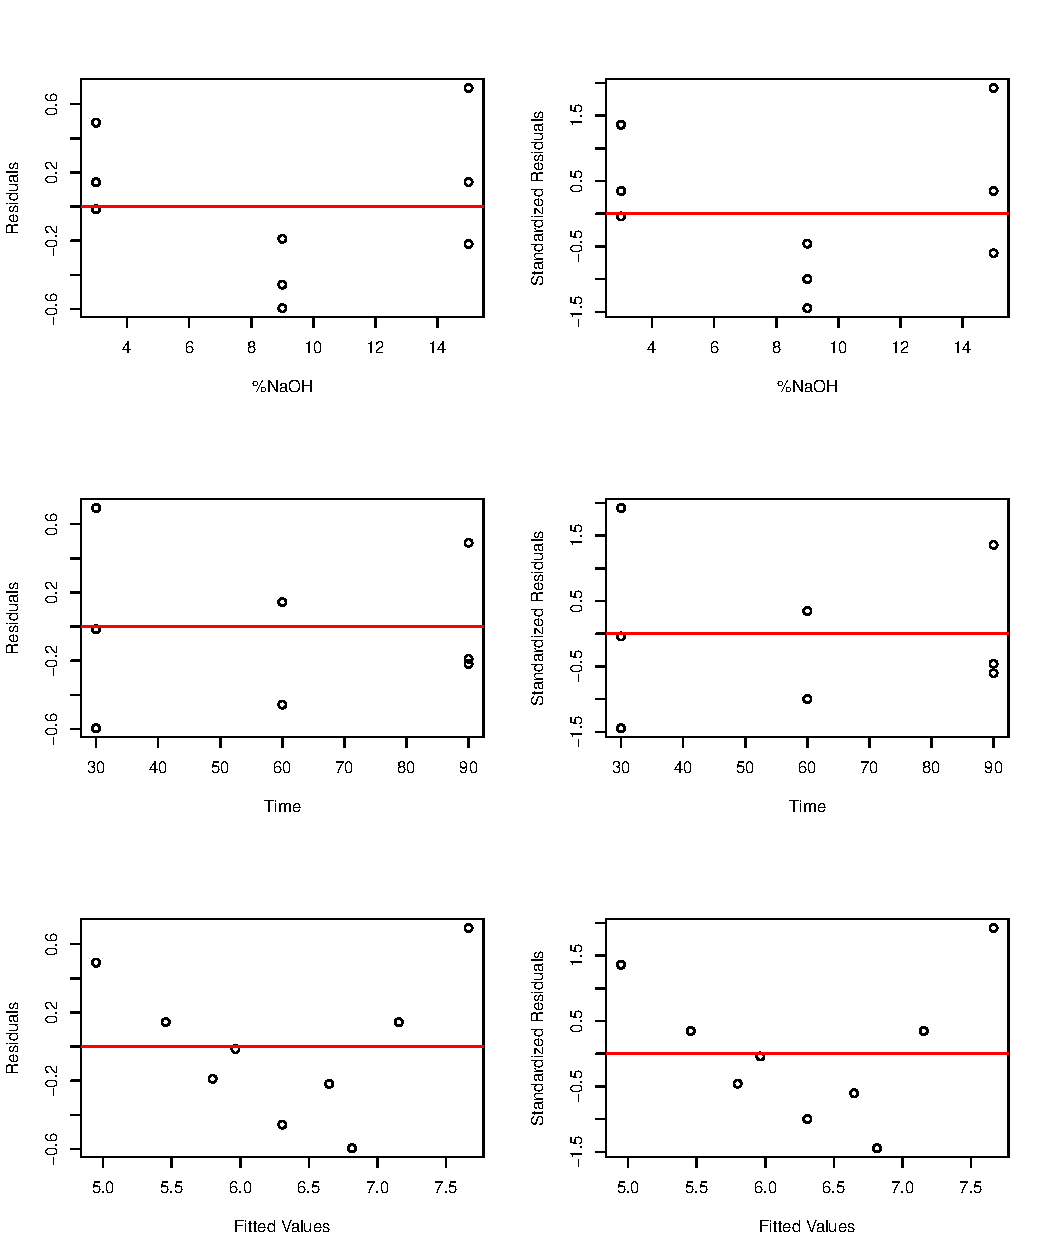
\includegraphics[width=0.8\textwidth]{figure/unnamed-chunk-3-1} 

}



\end{knitrout}
  
  For each of teh three types of plots, the residuals and standardized residuals look almost exactly the same.
  
  \item[(c)] The quantile used is $t_{6, 0.95} = 1.943$.
  
  The interval for $\beta_0$ is
  \[b_0 \pm t_{6, 0.95} \cdot se(b_0) = 6.0483 \pm 1.943(0.5208) = 6.043 \pm 1.011914 = (5.04, 7.06)\]
  
  The interval for $\beta_1$ is
  \[b_1 \pm t_{6, 0.95} \cdot se(b_1) = 0.14167 \pm 1.943(0.03301) = 0.14167 \pm 0.6413843 = (0.078, 0.206)\]
  
  The interval for $\beta_2$ is
  \[b_2 \pm t_{6, 0.95} \cdot se(b_2) = -0.016944 \pm 1.943(0.006601) = -0.016944 \pm 0.01282574 = (-0.0298, -0.0041)\]
  
  \item[(d)] The quantile used is $t_{6, 0.95} = 1.943$.
  
  For $x_1 = 9, x_2 = 60$, from the JMP saved column we have $\hat{\mu}_{y|\bm x} = 6.30667,\, se(\hat{\mu}_{y|\bm x}) = 0.162$. So the interval is
  \[\hat{\mu}_{y|\bm x} \pm t_{6, 0.95} se(\hat{\mu}_{y|\bm x}) = 6.30667 \pm 1.943(0.162) = 6.30667 \pm 0.314766 = (5.99, 6.62)\]
  
  For $x_1 = 10, x_2 = 70$, from the JMP saved column we have $\hat{\mu}_{y|\bm x} = 6.279,\, se(\hat{\mu}_{y|\bm x}) = 0.178$. So the interval is
  \[\hat{\mu}_{y|\bm x} \pm t_{6, 0.95} se(\hat{\mu}_{y|\bm x}) = 6.279 \pm 1.943(0.178) = 6.279 \pm 0.345854 = (5.93, 6.62)\]
  
  \item[(f)]
  The quantile for the one-sided 90\% prediction interval is $t_{6, 0.9} = 1.440$. From the JMP output, the lower prediction bound for $x_1 = 9, x_2 = 60$
  \begin{align*}
  &\hat{\mu}_{y|\bm x} - t_{6, 0.9} \sqrt{s_{SF}^2 + (se(\hat{\mu}_{y|\bm x}))^2}\\
  =&  6.30667 - 1.440 \sqrt{(0.4851)^2 + (0.162)^2}\\
  =& 6.30667 - 0.7364668 \\
  =& 5.57
  \end{align*}
  
  For $x_1 = 10, x_2 = 70$
  \begin{align*}
  &\hat{\mu}_{y|\bm x} - t_{6, 0.9} \sqrt{s_{SF}^2 + (se(\hat{\mu}_{y|\bm x}))^2}\\
  =&  6.279 - 1.440 \sqrt{(0.4851)^2 + (0.178)^2}\\
  =& 6.279 - 0.7440858 \\
  =& 5.53
  \end{align*}
  
  \item[(h)] The ANOVA table is shown below.
  
  \begin{center}
  \begin{tabular}{lrrrr}
  \hline
  Source & df & SS & MS & F \\ \hline
  Regression & 2 & 5.8854 & 2.9427 & 12.51\\
  Error & 6 & 1.4118 & 0.2353 &\\ \hline
  Total & 8 & 7.2972 & & \\ \hline
  \end{tabular}
  \end{center}
  
  The p-value is
  \[P(F_{2, 6} > 12.51) = 0.007242\]
  
  The p-value is very small, so this is very strong evidecne that the model used is an improvement over a model which does not depend at all on NaOH and Time ($y = \beta_0 + \epsilon$).
  
	\end{itemize}
	
	
	\item P. 724: 7 (ignore (f)) (5 points for each question) , dataset: {\tt grain\_thresher.jmp} 
	

	
	\begin{enumerate}
	\item
	From the JMP output, $s_{SF} = 0.3471$. Assuming that the model is appropriate, this measures the variation in Weights for a fixed Spacing. Using equation (7.7) in the textbook for the pooled sample variance, $s_{P} = 0.3448$. These two estimates are very close, giving no indication that the model is inappropriate.
	
	\item
	\begin{enumerate}[label = \arabic*.]
	\item
	$H_0: \beta_1 = \beta_2  = 0,\, H_a: $ not all of $\beta_1, \beta_2$ are 0
	\item
	The test statistic is
	\[F = \frac{SSR/(p-1)}{SSE/(n - p)} = \frac{SSR/2}{SSE/77}\]
	Assuming $H_0$ is true and the model $y = \beta_0 + \beta_1 x + \beta_2 x^2 + \epsilon$ is correct, the test statistic $F \sim F_{2, 77}$.
	\item
	From the JMP output, the observed $F$ is 18.64 and the p-value is 
	\[P(F_{2, 77} > 18.64) < 0.0001.\]
	\item
	The p-value is very small, so we reject $H_0$ and conclude $H_a$.
	\item
	There is overwhelming evidence that the model used is an improvement over a model in which Weight does not depend on Spacing ($y = \beta_0 + \epsilon$).
	\end{enumerate}
	
	\item
	\begin{enumerate}[label = \arabic*.]
	\item
	$H_0: \beta_2 = 0,\, \beta_2 \neq 0$
	\item
	The test statistic is
	\[T = \frac{b_2 - 0}{se(b_2)}\]
	Assuming $H_0$ is true and the model $y = \beta_0 + \beta_1 x + \beta_2 x^2 + \epsilon$ is correct, the test statistic $T \sim t_{77}$.
	\item
	The observed test statistic $t = -6.10$. The p-value is 
	\[P(|T| > |-6.10|) = 2P(T > 6.10) < 0.0001\]
	\item
	The p-value is very small, so we reject $H_0$ and conclude $H_a$.
	\item
	There is overwhelming evidence that the quadratic model is an improment over the straight-line model $y = \beta_0 + \beta_1 x + \epsilon$.
	\end{enumerate}
	
	\item
	For the one-sided 90\% confidence interval, we use $t_{77, 0.9} = 1.2926$. For $x = 1$, the 90\% lower confidence bound is
	\begin{align*}
  &\hat{\mu}_{y|\bm x} - t_{77, 0.9} se(\hat{\mu}_{y|\bm x}\\
  =&  13.0944 - 1.2926 (0.526)\\
  =& 13.0944 - 0.6799076 \\
  =& 13.03
  \end{align*}
	
	\item
	The quantile used is still $t_{77, 0.9} = 1.2926$. The lower prediction bound at $x = 1$ is
	\begin{align*}
  &\hat{\mu}_{y|\bm x} - t_{77, 0.9} \sqrt{s_{SF}^2 + (se(\hat{\mu}_{y|\bm x}))^2}\\
  =&  13.0944 - 1.2926 \sqrt{(0.3471)^2 + (0.0526)^2}\\
  =& 13.0944 - 0.4537839 \\
  =& 12.64
  \end{align*}
	\end{enumerate}
\end{enumerate}
%\newpage 
%\nocite{*}
%\bibliographystyle{plainnat} 
%\bibliography{}
\end{document}
